\documentclass[hyperref]{article}
%MS%%%%%%%%%%%%%%%%%%%% Article Format %%%%%%%%%%%%%%%%%
%+++++++++++++++++++++ Usepackage +++++++++++++++%%
\usepackage{graphicx} %% Package for Figure
\usepackage{float} %% Package for Float
\usepackage{amssymb}
\usepackage{amsmath}
\usepackage{mathtools}
\usepackage[thmmarks,amsmath]{ntheorem} %% If amsmath is applied, then amsma is necessary
\usepackage{bm} %% Bold Mathematical Symbols
\usepackage[colorlinks,linkcolor=cyan,citecolor=cyan]{hyperref}
\usepackage{extarrows}
\usepackage[hang,flushmargin]{footmisc} %% Let the footnote not indentation
\usepackage[square,comma,sort&compress,numbers]{natbib} %% Sort of References
\usepackage{mathrsfs} %% Swash letter
\usepackage[font=footnotesize,skip=0pt,textfont=rm,labelfont=rm]{caption,subcaption} 
%% Format of Caption for Tab. and Fig.
\usepackage{booktabs} %% tables with three lines
\usepackage{tocloft}
\usepackage{graphicx}
%+++++++++++++++ Proof etc. +++++++++++++++++++++++++%%
{%% Environment of Proof
	\theoremstyle{nonumberplain}
	\theoremheaderfont{\bfseries}
	\theorembodyfont{\normalfont}
	\theoremsymbol{\mbox{$\Box$}}
	\newtheorem{proof}{Proof}
}

\usepackage{theorem}
\newtheorem{theorem}{Theorem}[section]
\newtheorem{lemma}{Lemma}[section]
\newtheorem{definition}{Definition}[section]
\newtheorem{assumption}{Assumption}[section]
\newtheorem{example}{Example}[section]
\newtheorem{corollary}{Corollary}[section]
{%% Environment of Remark
	\theoremheaderfont{\bfseries}
	\theorembodyfont{\normalfont}
	\newtheorem{remark}{Remark}[section]
}
\usepackage{abstract}
\renewcommand{\abstractnamefont}{\Large\bfseries}
%\numberwithin{equation}{section} %% Number of Equation
%++++++++++++++++++++++++++++++++ Page format ++++++++++++++++++++++++++%%
\graphicspath{{figure/}}                                 %% Path of Figures
\usepackage[a4paper]{geometry}                           %% Paper size
\geometry{left=2.5cm,right=2.5cm,top=2.5cm,bottom=2.5cm} %% Margin
\linespread{1.2}                                         %% Line Spread
%MS%%%%%%%%%%%%%%%%%%%%%%%%%%%% End Format %%%%%%%%%%%%%%%%%%%%%%%%%%%%%%%%%%

%MS%%%%%%%%%%%%%%%%%%%%%%%%%%%%%%%%%%%%%%%%%%%
%MS                                         %%
%MS        The Main Body begins here        %%
%MS                                         %%
%MS%%%%%%%%%%%%%%%%%%%%%%%%%%%%%%%%%%%%%%%%%%%

%MS++++++++++++++++++++++++++++++ Title +++++++++++++++++++
\title{Assignment for EE5101/ME5401 Linear Systems}
\author{\textup{Yihui Chen}}
\begin{document}
	\begin{titlepage}
		\center
		\newcommand{\HRule}{\rule{\linewidth}{0.5mm}}
		
\includegraphics[width=8cm]{logo.png}\\[1cm] 
		\quad\\[1.5cm]
		\textsl{\Large National University of Singapore}\\[0.5cm] 
		\textsl{\large College of Design and Engineering}\\[0.5cm]
		\makeatletter
		\HRule \\[0.4cm]
		{ \huge \bfseries \@title}\\[0.4cm] 
		\HRule \\[1.5cm]
		\begin{minipage}{0.4\textwidth}
			\begin{flushleft} \large
				\emph{Author:}\\
				\@author 
			\end{flushleft}
		\end{minipage}
		~
		\begin{minipage}{0.4\textwidth}
			\begin{flushright} \large
				\emph{Supervisor:} \\
				\textup{Prof Yang}
			\end{flushright}
		\end{minipage}\\[3cm]
		\makeatother
		{\Large Assignment for EE5101/ME5401 Linear System}\\[0.5cm]
		{\large \emph{Matriculation Number: A0263115N}}\\[0.5cm]
		{\large \emph{Email Address: e1010473@u.nus.edu}}\\[0.5cm]
		{\large \today}\\[2cm] 
		\vfill 
	\end{titlepage}
	

	%MS+++++++++++++++++++++ Abstract +++++++++++++++++++++++++
	\begin{abstract}
		
	This is abstract
	
	Plant description
	Control and observer design method description
	Design details
	Simulation results
	Possible comparison
	Comments and discussion
	Modification and refinements
	
	\end{abstract}
	
	\vspace{1ex}
	{\noindent\small{\bf Keywords:}
		Keywords1; Keywords2;...}
	
	\newpage
	
	\tableofcontents
	\newpage
	
	%MS++++++++++++++++++++++++++++++ Main body ++++++++++++++++++++
	\section{Introduction}
	
	Combining the high safty of car and low cost of motor, self-sustaining two-wheeled vehicle (Fig.~\ref{fig1}) has drawn research interest in universities. Though most of study are still in experimental stage, different control methods have been tested on this mortorcycle-like vehicle and some exprimental results have been released online. 
	
	\begin{figure}[htbp]
		\centering
		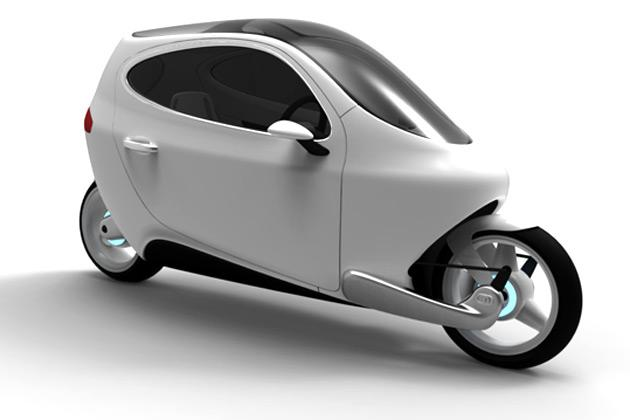
\includegraphics[width=0.4\linewidth]{fig1.png}
		\caption{Two-wheeled self-balancing car}
		\label{fig1}
	\end{figure} 
	
	The two-wheeled vehicle is composed of a cart system, a steering system (front part) and a body (rear part). Driven by the DC servo motor, the cart and steering systems allow drivers to change cart position and handle angle. To simplify the modeling in this mini-project, the self-balance two-wheeled vehicle is assumed to be stationary and the mechanical structure is given in Fig.~\ref{fig2}.
	
	\begin{figure}[htbp]
		\centering
		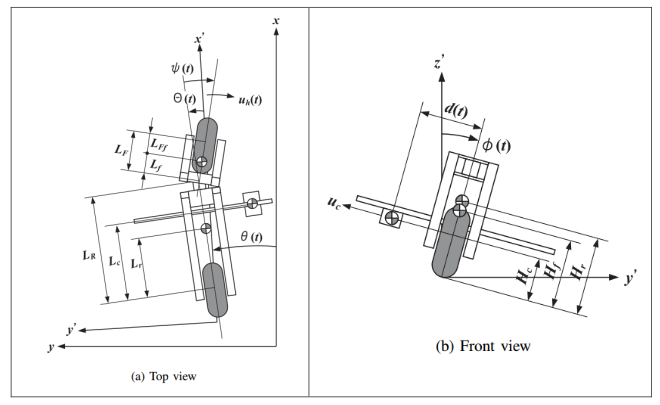
\includegraphics[width=0.6\linewidth]{fig2.png}
		\caption{Simple two-wheeled vehicle model}
		\label{fig2}
	\end{figure} 
	
	Then, state space model is established
	
	\begin{equation}
	\begin{split}
	\begin{aligned}
		\dot{x}&=Ax+Bu \\
		y&=Cx
	\label{eq1}
	\end{aligned}
	\end{split}
	\end{equation}
	
	where the state is designed according to the cart position, handle angle, bike angle and their corresponding velocities respectively
	
	\begin{equation}
		x=\begin{bmatrix}
		d(t) & \phi(t) & \psi(t) & \dot{d}(t) & \dot{\phi}(t) & \dot{\psi}(t) 
		\end{bmatrix}^{T}
	\label{eq2}
	\end{equation}
	
	and the relative matrices and input vectors are
	
	\begin{equation}
		A=\begin{bmatrix}
		0 &0  &0  &1  &0  &0 \\ 
		0 &0  &0  &0  &1  &0 \\ 
		0 &0  &0  &0  &0  &1 \\ 
		0 &6.5  &-10  &-\alpha   &0  &0 \\ 
		a_{51} &a_{52}  &a_{53}  &a_{54}  &a_{55}  &a_{56} \\ 
		5 &-3.6  &0  &0  &0  &-\gamma  
		\end{bmatrix}, 
		B=\begin{bmatrix}
		0 &0 \\ 
		0 &0 \\ 
		0 &0 \\ 
		\beta  &11.2 \\ 
		b_{51} &b_{52} \\ 
		40 &\delta  
		\end{bmatrix}
	\label{eq3}
	\end{equation}
	
	\begin{equation}
		C=\begin{bmatrix}
		1 &0  &0  &0  &0  &0 \\ 
		0 &1  &0  &0  &0  &0 \\ 
		0 &0  &1  &0  &0  &0 
		\end{bmatrix},
		D=\begin{bmatrix}
		u_{c}(t) &u_{h}(t) 
		\end{bmatrix}^{T}
	\label{eq4}
	\end{equation}
	
	The parameters in matrix $A$ and $B$ can be calculated as
	
	\begin{equation}
		%\begin{gather}
	\begin{split}
			a_{51}&=-\frac{M_{c}g}{den},
			a_{52}=\frac{(M_{f}H_{f}+M_{r}H_{r}+M_{c}H_{c})g}{den}, 
			a_{53}=\frac{(M_{r}L_{r}L_{F}+M_{c}L_{c}L_{F}+M_{f}L_{Ff}L_{R})g}{(L_{R}+L_{F})den}\\
			a_{54}&=-\frac{M_{c}H_{c}\alpha}{den},
			a_{55}=-\frac{\mu _{x}}{den},
			a_{56}=\frac{M_{f}H_{f}L_{Ff}\gamma }{den}\\		
			b_{51}&=\frac{M_{c}H_{c}\alpha }{den},
			b_{52}=-\frac{M_{f}H_{f}L_{Ff}\delta }{den},
			den=M_{f}H_{f}^{2}+M_{r}H_{r}^2+M_{c}H_{c}^{2}+J_{x}
			\label{eq5}			
		%\end{gather}
	\end{split}
	\end{equation}
	
	The physical parameters appering in Eq.~\ref{eq4} and Eq.~\ref{eq5} are usually measured mannually by experiments and they are given in appendix.
	
	After obtaining the linear system model and giving a step reference signal for each input channel, two basic response performance specifications are required to meet as follows
	
	\begin{itemize}
		\item The overshoot of system should below 10\%.
		\item The 2\% settling time should be less than 5 seconds.
	\end{itemize}

	The rest of the report is structured in the following manner: In section 2 a state feedback controller is designed using pole placement methods, followed by a discussion on effects of different pole choices. Section 3 concludes a Linear Quadratic Regulator controller design as well as the techique on choosing the weighting matrixes $Q$ and $R$. Section 4 introduces a state observer based on the former LQR control system and its performance is evaluated by monitoring the state estimation error. Section 5 describes a decoupling controller for a 2-input-2-output system. Section 6 designes a controller enabling the output of plant to track the reference signal regardless of step disturbances in input channel. Section 7 tries the integral control method to maintain outputs at a constatnt set point with zero steady-state error. Section 8 concludes the work.
	
	\section{State feedback controller by pole placement method}
	
	\subsection{Method description}
	
	\hspace{1.0em}
	Given the acquired six-order state space model, feedback controller is required to make the system stable. In this section, pole placement method will be used to obtain the feedback gain to meet control requirements. Firstly considering a second-order system, its overshoot and 2\% settling time of a step response is given as follows
	
	\begin{equation}
	M_{p}=e^{\frac{-\pi \zeta }{\sqrt{1-\zeta ^{2}}}}, t_{s}=\frac{4.0}{\zeta \omega _{n}}
	\label{eq6}
	\end{equation}
	
	where $\zeta$ and $\omega_{n}$ are damping ratio and natural frequency respectively. Now that the overshoot should below 10\% and settling time less than 5s, we set $\zeta=0.8$ and $\zeta\omega_{n}=2.5$ in this case, and then the two pole of second-order system is calculated as
	
	\begin{equation}
	\lambda _{1,2}=-\zeta \omega _{n}\pm j\omega _{n}\sqrt{1-\zeta ^{2}}
	\label{eq7}
	\end{equation}
	
	To assure the stability of system, the two dominant poles should have little smaller real parts, so we set them at $\lambda_{1,2}=-2.5\pm j1.875$. The other 4 poles are chosen 4-5 times lefter than the two dominant poles. Then the desired characteristic polynomial becomes
	
	\begin{equation}
	\begin{split}
	\begin{aligned}
		\phi _{d}(s)&=(s-\lambda _{1})(s-\lambda _{2})(s-\lambda _{3})(s-\lambda _{4})(s-\lambda _{5})(s-\lambda _{6})\\
		&=s^{6}+a_{5}s^{5}+a_{4}s^{4}+a_{3}s^{3}+a_{2}s^{2}+a_{1}s+a_{0}
	\end{aligned}
	\end{split}
	\label{eq8}
	\end{equation}
	
	The desired closed-loop matrix can be written in controllable canonical form
	
	\begin{equation}
	A_{d}=\begin{bmatrix}
	0 &  1&0  &0  &0  &0 \\ 
	0 &0  &1  &0  &0  &0 \\ 
	0 &0  &0  &1  &0  &0 \\ 
	0 &0  &0  &0  &1  &0 \\ 
	0 &0  &0  &0  &0  &1 \\ 
	-a_{5} &-a_{4}  &-a_{3}  & -a_{2} &-a_{1}  & -a_{0}
	\end{bmatrix}
	\label{eq9}
	\end{equation}
	
	Then the remainning task is transform the system with state feedback also to the controllable canonical form. First compute the controllability matrix and check if it is full rank
	
	\begin{equation}
	W_{c}=\begin{Bmatrix}
	B &AB  &A^{2}B  &A^{3}B &A^{4}B  & A^{5}B
	\end{Bmatrix}
	\label{eq10}
	\end{equation}
	
	Then select 6 independent vectors from $W_{c}$ in the strict order from left to right (the first six column vectors in this case) and group them in matrix X in the following form
	
	\begin{equation}
	X=\begin{Bmatrix}
	b_{1} &b_{2}  &Ab_{1}  &Ab_{2}  &A^{2}b_{1}  &A^{2}b_{2} 
	\end{Bmatrix}
	\label{eq11}
	\end{equation}
	
	Also compute the inverse of $X$ and write it as the following form
	
	\begin{equation}
	X^{-1}=\begin{bmatrix}
	q_{1}^{T} & q_{2}^{T} & q_{3}^{T} & q_{4}^{T} & q_{5}^{T} & q_{6}^{T}
	\end{bmatrix}^{T}
	\label{eq12}
	\end{equation}
	
	Because that the system has multiple input channels, choose the $3^{th} (d_{1}=3)$ and $6^{th} (d_{1}+d_{2}=6)$ row vectors of $X^{-1}$ and construct transformation matrix $T$ as
	
	\begin{equation}
	T=\begin{bmatrix}
	q_{3}^{T} &q_{3}^{T}A  &q_{3}^{T}A^{2}  & q_{6}^{T} &q_{6}^{T}A  &q_{6}^{T}A^{2}
	\end{bmatrix}^{T}
	\label{eq13}
	\end{equation}
	
	Define the feedback gain matrix $\bar{K}\in \mathbb{R}^{2\times 6}$ with 12 unknown variables, we can solve it by establishing the equation
	
	\begin{equation}
	\bar{A}-\bar{B}\bar{K}=A_{d}
	\label{eq14}
	\end{equation}
	
	where $\bar{A}=TAT^{-1}$, $\bar{B}=TB$
	
	After obtainning the matrix $\bar{K}$, we can finally get the original feedback gain matrix $K=\bar{K}T$. Substitute the control law $u=-Kx+r$ into Eq.~\ref{eq1} and the new closed-loop system becomes
	
	\begin{equation}
	\begin{split}
	\begin{aligned}
	\dot{x}&=(A-BK)x+Br \\
	y&=Cx
	\label{eq15}
	\end{aligned}
	\end{split}
	\end{equation}
	
	
	\subsection{Simulation results and refinements}
	
	\hspace{1.0em}
	In this report, the 6 poles are selected as $\lambda_{1,2}=-2.5\pm j1.875, \lambda_{3}=-10, \lambda_{4}=-10.75, \lambda_{5}=-11.5$ and $\lambda_{6}=-12.5$. The final feedback gain matrix $K$ is calculated to be
	
	\begin{equation}
	K=\begin{bmatrix}
	-15.68 &12.20  &6.27  &4.90  &-6.21  &-2.26 \\ 
	250960 &-21110  &-107660  &-845.58  &9043.2  &412.98 
	\end{bmatrix}
	\nonumber
	\end{equation}
	
	The number of elements differes a lot and are relatively weird. Temporarily we use the feedback matrix and simulate the closed-loop system with time domain from 0 to 10 seconds. Given a step signal for each input channel, the output response is showed in Fig.~\ref{fig3}. Sadly though the system becomes stable with a short settling time, there are huge overshoots in both cases and the stable points are also impossible in real cases. 
	
	\begin{figure}[htbp]
		\centering
		\begin{minipage}[t]{0.48\textwidth}
			\centering
			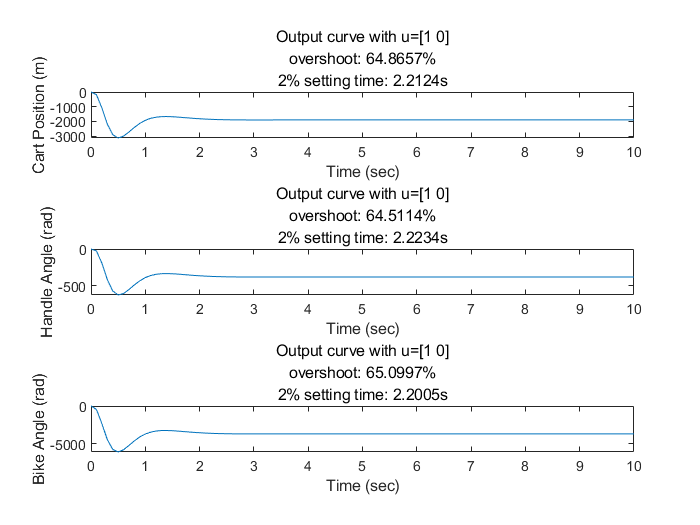
\includegraphics[width=8cm]{fig3.png}
		\end{minipage}
		\begin{minipage}[t]{0.48\textwidth}
			\centering
			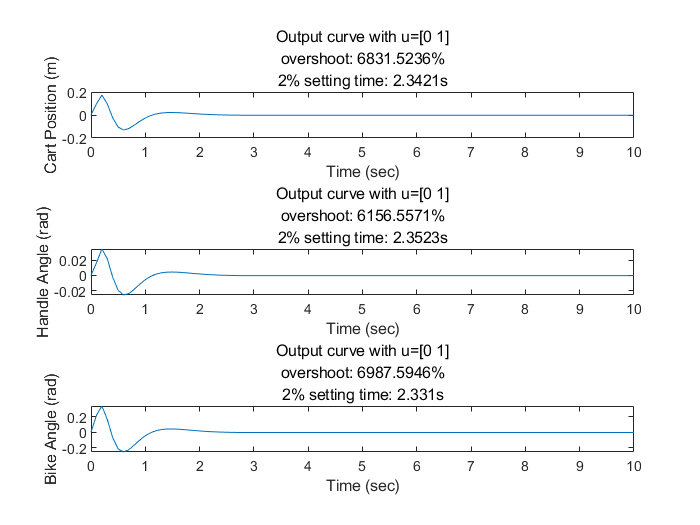
\includegraphics[width=8cm]{fig4.png}
		\end{minipage}
	\caption{Step response for the closed-loop system}
	\label{fig3}
	\end{figure}
	
	The results are unacceptable and need further refinements. Obviously, the bad results are closely realted to the feedback gain matrix $K$, which influnces the system matrix $A-BK$ of closed-loop system. In another point of view, we can find infinite $K$ to place the same poles for a plant as there are infinite system matrixes with the same eigenvalues. 
	
	Actuallly when tackling pole placement problems for high order system, some pole choices will result in sensitivity problems, which leads to a large gain as in our former method. One robust algorithm was proposed in \cite{kautsky1985robust} and has been applied in matlab function. The aim of this algorithm is to find the feedback gain matrix $K$ that makes $A-BK$ the most robust. One method to measure the robustness of a matrix is to use condition number
	
	\begin{equation}
	c_{j}=\frac{1}{s_{j}}=\frac{\left \| y_{j} \right \|_{2} \left \| x_{j} \right \|_{2}}{\left |y_{j}^{T} x_{j}  \right |}
	\label{eq16}
	\end{equation}
	
	where $x_{j}$ and $y_{j}$ are the left and right eigenvalues of $A-BK$ respectively. It can be proved that $c_{j}$ has a upper bound i.e. $max_{j}c_{j} \leq \kappa _{2}(X)\equiv \left \| X \right \|_{2}\left \| X^{-1} \right \|_{2}$, where $X=\begin{bmatrix}
	x_{1} &x_{2}  &\cdots   & x_{n}
	\end{bmatrix}$ is the eigenvector matrix. The maximum value $v=max(c_{j})$ of all condition numbers is chosen and the system is said to be the most robust if $v$ is the smallest. Then the problem becomes how to find the minimum upper bound of condition numbers.
	
	The minimum upper bound can ben found by cauchy inequality and the result is given as follows
	
	\begin{equation}
	min ( \kappa _{2}(X)) \leq \frac{\kappa _{2}(S)}{\sqrt{k}}
	\label{eq17}
	\end{equation}
	
	$S$ is orthogonal normal basis of the null space of $N(U_{1}^{T}(A-\lambda I))$, where $U_{1}$ is the orthogonal basis of null space of input matrix $B$, $\lambda$ are eigenvalues of matrix $A-BK$ and $k$ is the dimensions of $S$. QR decomposition or singular value decomposition (SVD) can be used to calculate the orthogonal basis. Finally, feedback gain matrix $K$ can be obtained by
	
	\begin{equation}
	K=Z^{-1}U_{0}^{T}(A-X\Lambda X^{-1})
	\label{eq18}
	\end{equation}
	
	where $\Lambda=diag(\lambda_{1},\lambda_{2},...,\lambda_{n})$, $Z$ is the $Q$ matrix of $B$ and $U_{0}$ is also orthogonal basis of $B$.
	
	The same poles are chosen but we use the new method to calculate feedback matrix ${K}'$, the result is given below
	
	\begin{equation}
	{K}'=\begin{bmatrix}
	8.7165 &-3.6746  &-1.8207  &0.5685  &-0.4985  &-0.0880 \\ 
	-11.2971 &10.6474  &5.4543  &-0.8739  &1.4368  &0.3794 
	\end{bmatrix}
	\nonumber
	\end{equation}
	
	The step response for the new closed-loop system is shown in Fig.~\ref{fig4} and both the overshoot and settling time meet the requirements. Now assume that all six states can be observed, their response with non-zero initial condition $x_{0}$ to zero external inputs is given in Fig.~\ref{fig5}. It is clearly shown that all states are stable and no weired values apper.
	
	\begin{figure}[htbp]
		\centering
		\begin{minipage}[t]{0.48\textwidth}
			\centering
			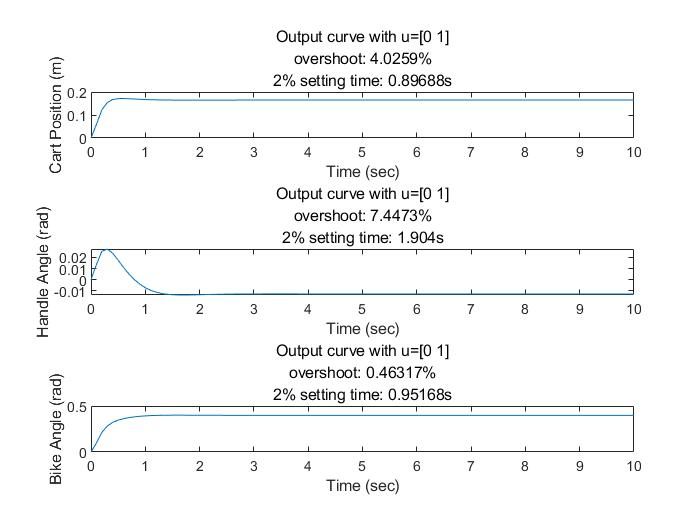
\includegraphics[width=8cm]{fig5.png}
		\end{minipage}
		\begin{minipage}[t]{0.48\textwidth}
			\centering
			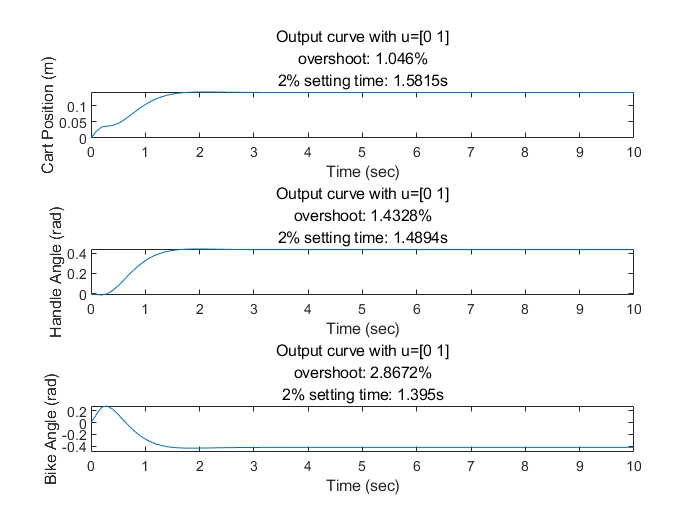
\includegraphics[width=8cm]{fig6.png}
		\end{minipage}
		\caption{Step response for the new closed-loop system}
		\label{fig4}
	\end{figure}

	\begin{figure}[htbp]
		\centering
		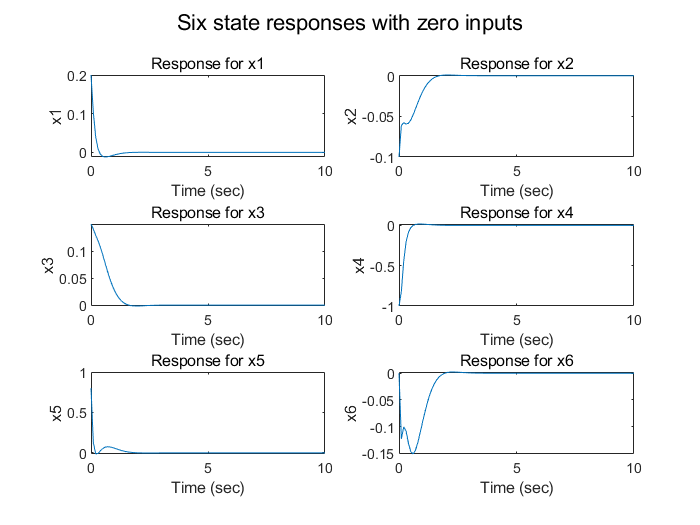
\includegraphics[width=0.8\linewidth]{fig7.png}
		\caption{All state responses with zero inputs}
		\label{fig5}
	\end{figure} 
	
	\subsection{Discussion}
	
	\hspace{1.0em}
	With refinements on feedback gain matrix $K$, the overshoot of the closed-loop system is largely cut down as well as its sensitivity to noise. On the other side, the system performance is also largely affected by different pole choosing strategies. Although one can always stablize the system and make system response faster by designing poles on the very left plain, the input cost will increase in this case. To investigate the influence of poles, two more groups of poles are used. The new poles are listed as followings
	
	\begin{equation}
	\begin{split}
	\begin{aligned}
	{p}'&= \begin{bmatrix}
	-1.6+j0.96 &-1.6-j0.96  &-6.4  &-6.88  &-7.36  &-8
	\end{bmatrix}\\
	{p}''&= \begin{bmatrix}
	-4+j3 &-4-j3  &-16  &-17.2  &-18.4  &-20 
	\end{bmatrix}
	\end{aligned}
	\end{split}
	\nonumber
	\end{equation}
	
	It is clearly shown in Fig.~\ref{fig6}, \ref{fig7} and \ref{fig8} that the larger negative real parts the pole has, the more control effect is required. However if the designed poles are too right, large overshoot or long settling time may be expected to appear (as is shown in Fig.~\ref{fig9}).
	
	\begin{figure*}[htbp] %通栏
		\begin{minipage}[t]{0.33\linewidth} %调节两个子图左右间距
			\centering
			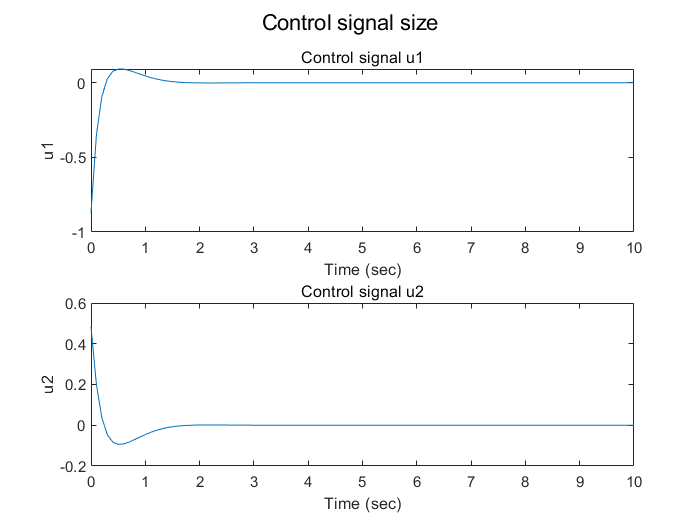
\includegraphics[width=2.5in, height=1.9in]{fig8.png} %调节单个子图大小
			\caption{Control signal size with $p$} %子图下标题
			\label{fig6}
		\end{minipage}%
		\begin{minipage}[t]{0.33\linewidth}
			\centering
			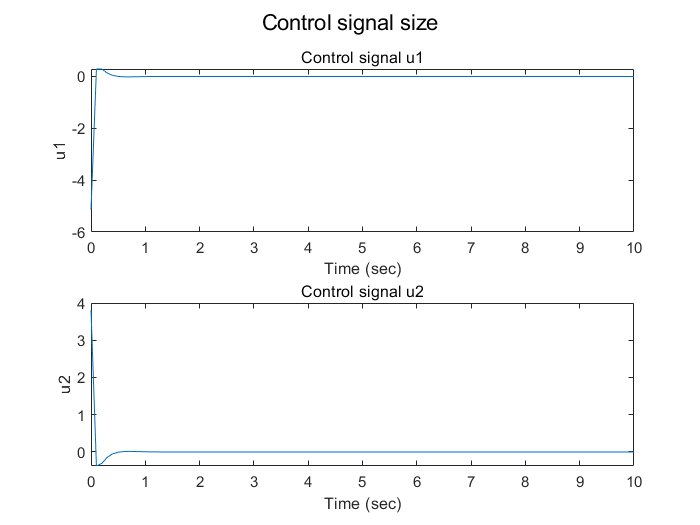
\includegraphics[width=2.5in, height=1.9in]{fig9.png}
			\caption{Control signal size with ${p}'$}
			\label{fig7}
		\end{minipage}%
		\begin{minipage}[t]{0.33\linewidth}
			\centering
			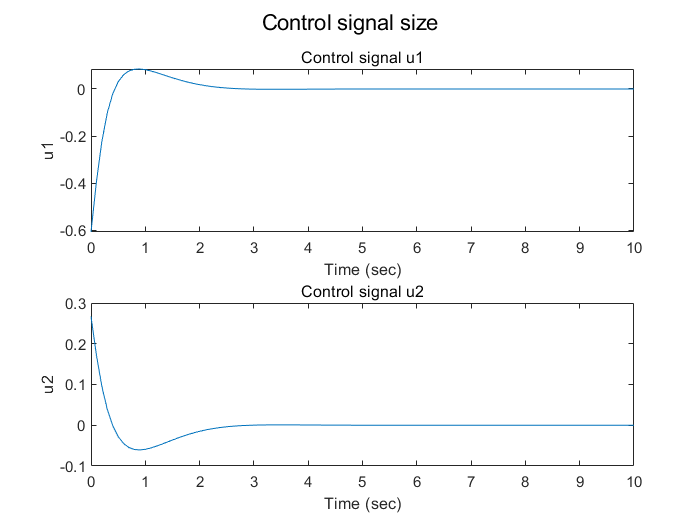
\includegraphics[width=2.5in, height=1.9in]{fig10.png}
			\caption{Control signal size with ${p}''$}
			\label{fig8}
		\end{minipage}
	\end{figure*}

	\begin{figure}[htbp]
		\centering
		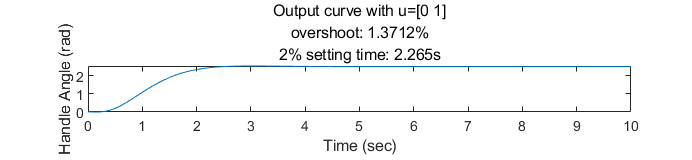
\includegraphics[width=0.6\linewidth]{fig11.png}
		\caption{Large overshoot show when given ${p}''$ with small negative real parts}
		\label{fig9}
	\end{figure}
	
	Pole placement methods have the magic of easily stabilizing the system and ensuring the expected design performance by using state feedback controller. On the other hand, poles of systems are hard to select and have no strict standards. In next section, linear quadratic regulator will be introduced to solve the trade-off problem between system performance and control cost.
	
	
	\section{Linear quadratic regulator controller}
	...
	\section{Conclusion}
	\section*{Acknowledgments}
	%MS++++++++++++++++++++++++++++++ Reference ++++++++++++++++++
	%% 参考文献请看下一节详细介绍。
	
	\bibliographystyle{IEEEtran}
	
	\bibliography{ref_5401}{}
	
\end{document}